\section{Algoritmo di Karger}\label{karger}
\begin{lstlisting}[mathescape=true]
KARGER(G, k):

	min = +$\infty$
	for i = 1 to k:		
		t = FULL_CONTRACTION(G)		
		if t < min:
			t = min
			
	return min

FULL_CONTRACTION(G):

	for i = 1 to |V|-2:
		pick a random edge e = (u, v)
		merge u and v in a single node
		remove edges between u and v
		
	return |E| // the edges between the two remaining vertices (u* ,v*)
\end{lstlisting}	

L'algoritmo di \textit{Karger} è un algoritmo randomizzato per la computazione del \textit{minimum cut} di un multi-grafo connesso.\\
Un ``\textit{multi-grafo}'' è un particolare tipo di grafo che ammette ripetizioni di lati al suo interno, ovvero questi possono apparire più di una volta (con \textit{molteplicità} $\geq$ 1).\\
L'idea su cui si basa l'algoritmo qui implementato, è quella di contrarre i vertici all'interno del multi-grafo fino a quando non ne restano solamente due, i quali rappresentano gli opposti del taglio.\\
Per ``\textit{contrarre}'' si intende \textit{unire} i due nodi estremi di un lato in maniera da averne solamente uno. 
Dopo averli uniti vanno aggiustate le vecchie liste di adiacenza, unite in una singola, in maniera che i vecchi puntatori ai nodi tolti siano stati correttamente sostituiti con riferimenti al nuovo nodo e che non ci siano \textit{self-loops}.\\
Essendo che è un \textit{algoritmo randomizzato}, ovvero utilizza un grado di casualità come parte della sua logica, la procedura di contrazione va eseguito $k$ volte, con $k$ calcolato in maniera da soddisfare la probabilità:
\begin{center}
	$Pr("le~k~FULL\_C.~non~accumulano~la~taglia~del~min~cut") \leq (1-\frac{2}{n^2})^k$

\end{center}
Voglio ottenere qualcosa del tipo $\frac{1}{n^d}$ e quindi scelgo $k = d\frac{n^2}{2}\ln n$.\\
La logica che implementa la parte randomica in questo caso è la scelta del lato i cui nodi andranno contratti.\\
Possiamo quindi dire che l'algoritmo funziona con probabilità bassissima, che può però essere amplificata ripetendo questo processo molte volte, esattamente k.\\
Essendo però che questo potrebbe portare via tanto tempo da eseguire su tutte le istanze del dataset abbiamo introdotto un tempo massimo di 60 secondi per ciascuna istanza.

\subsection{Strutture dati}

	A differenza degli altri homework, per migliorare le performance dell'algoritmo in questione, abbiamo deciso di utilizzare solamente la struttura dati \texttt{Graph}, implementata con i seguenti campi e metodi:
	\begin{itemize}
		\item \texttt{\textbf{n\_nodes}}: numero di nodi del grafo;
		\item \texttt{\textbf{n\_edges}}: numero di lati del grafo;
		\item \texttt{\textbf{nodes}}: dizionario con i nodi del grafo e le rispettive liste di adiacenza;
		\item \texttt{\textbf{edges}}: lista con i lati del grafo;
		\item \texttt{\textbf{\_\_init\_\_()}}: metodo di inizializzazione che imposta i precedenti campi a 0 o vuoti;
		\item \texttt{\textbf{addEdge(v1, v2)}}: metodo che dati due nodi aggiunge il lato che li unisce alla lista \texttt{edges};
		\item \texttt{\textbf{buildGraph(data)}} metodo che riceve in input una matrice di adiacenza e, in base a questa, ne costruisce un grafo.
	\end{itemize}
	
\subsection{Funzioni}
	
	Le funzioni ausiliarie utilizzate per calcolare la soluzione dell'algoritmo di Karger sono le seguenti:
	\begin{itemize}
		\item \texttt{\textbf{readInput(path)}}: metodo che, dato in input il path del dataset, ne legge il contenuto e restituisce la matrice di adiacenza del grafo;
		\item \texttt{\textbf{graphCopy(graph)}}: metodo che riceve in input un oggetto di tipo \texttt{Graph} e ne restituisce una copia;
		\item \texttt{\textbf{execute\_alg(path)}}: metodo che, dato in input il path del dataset, esegue la chiamata a \texttt{Karger(G)} calcolando i tempi richiesti nella consegna e confrontando i risultati ottenuti con quelli attesi.
	\end{itemize}

\subsection{Implementazione}
	
	La soluzione del problema è stata implementata nel seguente modo:
	\begin{itemize}
		\item a partire dalla lista di vertici nel file di input, viene costruito il grafo \texttt{graph};
		\item viene calcolato il valore \texttt{k} tramite la formula \texttt{int((graph.n\_nodes**2 / 2) * \\
			math.log(graph.n\_nodes))}. Se \texttt{k} supera $10000$ allora il suo valore lo fissiamo a tale soglia;
		\item per migliorare le performance della soluzione proposta, abbiamo deciso di creare in anticipo le copie dei grafi per ciascuna delle \texttt{k} volte che verrà eseguito \texttt{fullContraction(G)};
		\item viene effettuata la chiamata a \texttt{Karger(G,k)}, nel quale per \texttt{k} volte viene chiamato \texttt{fullContraction(G)}. I risultati di ciascuna chiamata vengono confrontati e viene salvato quello minimo, inoltre vengono registrati i tempi che sono presentati in formato tabellare nella Sez.~\ref{risultati}. Se il tempo di esecuzione supera quello massimo fissato, allora viene tornata la soluzione trovata fino a quel momento;
		\item per ciascuna chiamata a \texttt{fullContraction(G)}, questo metodo sceglie in maniera randomica un lato presente all'interno del grafo passato in input e unisce i vertici che ne rappresentano gli estremi in un singolo vertice. Per ciascuno degli altri vertici presenti all'interno del grafo si modificano le liste di adiacenza e aggiornando i riferimenti. Vengono inoltre diminuiti i contatori \texttt{n\_nodes} e \texttt{n\_edges} all'interno della struttura \texttt{Graph}. Questo metodo ritorna il numero rimanente di lati all'interno del grafo dopo aver eliminato $|V|-2$ nodi;
		\item i risultati vengono messi in coda alla lista e questo procedimento viene ripetuto per i rimanenti file in input non ancora valutati.
	\end{itemize}

	\vspace{1cm}
	\begin{center}
		\begin{figure}[H]
			\centering
			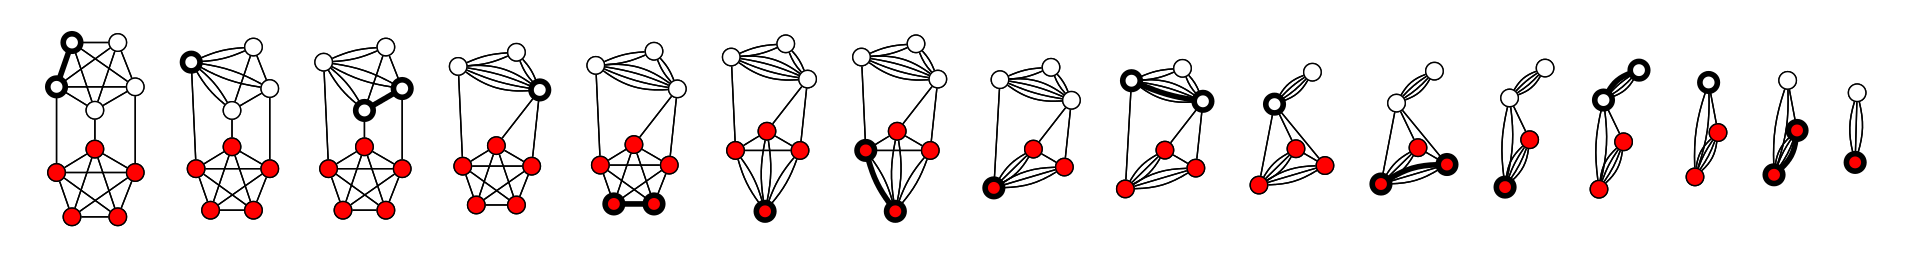
\includegraphics[width=\linewidth]{Img/example_1.png}
			\caption{Esempio di esecuzione dell'algoritmo di Karger e Full Contraption}
		\end{figure}
	\end{center}
	\vspace{-1cm}
		
\subsection{Complessità}

	Per calcolare la complessità di questo algoritmo bisogna tenere in considerazione:
	\begin{itemize}
		\item la complessità di Karger
		\item la complessità di fullContraction
	\end{itemize}
	La complessità totale dell'intero algoritmo risulta quindi essere

\pagebreak